% Created 2017-12-16 Sat 01:08
% Intended LaTeX compiler: pdflatex
\documentclass[11pt]{article}
\usepackage[utf8]{inputenc}
\usepackage[T1]{fontenc}
\usepackage{graphicx}
\usepackage{grffile}
\usepackage{longtable}
\usepackage{wrapfig}
\usepackage{rotating}
\usepackage[normalem]{ulem}
\usepackage{amsmath}
\usepackage{textcomp}
\usepackage{amssymb}
\usepackage{capt-of}
\usepackage{hyperref}
\usepackage{amsthm}
\usepackage{amsmath,amscd}
\usepackage{tikz-cd}
\newtheorem{remark}{Remark}
\newtheorem{theorem}{Theorem}
\newtheorem{lemma}[theorem]{Lemma}
\newtheorem{corollary}{Corollary}[theorem]
\newtheorem{conjecture}[theorem]{Conjecture}
\newtheorem{proposition}{Proposition}[theorem]
\newtheorem{problem}{Problem}
\newtheorem{exampl}{Example}
\newtheorem{definition}{Definition}
\newtheorem{propdef}[definition]{Proposition-Definition}
\newcommand{\im}{\mathop{\rm Im}\nolimits}
\newcommand{\supp}{\mathop{\rm supp}\nolimits}
\newcommand{\ord}{\mathop{\rm ord}\nolimits}
\newcommand{\Spec}{\mathop{\rm Spec}\nolimits}
\newcommand{\vol}{\mathop{\rm vol}\nolimits}
\newcommand\restr[2]{{% we make the whole thing an ordinary symbol
\left.\kern-\nulldelimiterspace % automatically resize the bar with \right
#1 % the function
\vphantom{\big|} % pretend it's a little taller at normal size
\right|_{#2} % this is the delimiter
}}
\author{darknmt}
\date{\today}
\title{Divisors, Picard group and Kodaira embedding theorem}
\hypersetup{
 pdfauthor={darknmt},
 pdftitle={Divisors, Picard group and Kodaira embedding theorem},
 pdfkeywords={},
 pdfsubject={},
 pdfcreator={Emacs 25.3.1 (Org mode 9.0.5)}, 
 pdflang={English}}
\begin{document}

\maketitle
\tableofcontents

\iffalse
\begin{info}
The PDF version of this page can be downloaded by replacing \texttt{html} in the its address by
\texttt{pdf}. 
For example \texttt{/html/sheaf-cohomology.html} should become \texttt{/pdf/sheaf-cohomology.pdf}.
\end{info}
\fi

\section{Divisors and Picard group}
\label{sec:org6ca8ed8}

\subsection{Holomorphic line bundles and first Chern class}
\label{sec:org7268523}

A \uline{complex line bundle} is a 2 dimensional vector bundle with a complex structure on each
fiber, i.e. each change of coordinates \(g_{ij}: U_j\cap U_i \times \mathbb{R}^2
\longrightarrow  U_i\cap U_j\times\mathbb{R}^2\) is \(i\)-linear, i.e. \(g_{ij}\) can
be represented by a function \(U_{i}\cap U_j \longrightarrow \mathbb{C}\). 

A \uline{holomorphic line bundle} is a complex line bundle that is also a complex manifold with
the projection being holomorphic. In the same notation, the \(g_{ij}\) are now
holomorphic functions.

A \uline{hermitian metric} on a line bundle \(L\) is a positive sesquilinear form on each
fiber. To define the \uline{Chern form} of \(L\), let \(U\) be an open set of \(X\) over
which \(L\) is trivialized and \(s_x\) is a holomorphic section of \(L\) over \(U\) that is
non-vanishing, then one defines
\[
\omega_{L,h} = \frac{1}{2\pi i}\partial \bar \partial \log |s|_h^2
\]
which is independant of \(s\) since the ratio of two different \(s\) is in \(\mathcal{O}^*(U)\).

\begin{remark}
A Chern form is a real (1,1) form.
\end{remark}


\begin{proposition}
The set of isomorphic class of holomorphic line bundle is in one-to-one correspondance to \(H^1(X,\mathcal{O}_X^*)\)
\end{proposition}

The proof of this fact is straightforward, but it is worth to remark that this result
convinces us that the natural mapping \(\check{H}^1(\mathcal{U},X) \longrightarrow
\check{H}^1(\mathcal{V},X)\) where \(\mathcal{U}\) is a finer open covering than \(\mathcal{V}\) is injective, since a line bundle is completely defined by \emph{one} set of
change of coordinates \((g_{ij})\).

Now the \uline{Chern class} of a holomorphic line bundle is the class of \(\omega_{L,h}\) in
\(H^2(X,\mathbb{Z})\), which turns out to be independent of \(h\) and is in fact lies
in the image of \(H^2(X,\mathbb{Z}) \longrightarrow H^2(X,\mathbb{R}) = H^2(X, \mathbb{Z})\otimes_{\mathbb{Z}}\mathbb{R}\). In fact, the class
of \(\omega_{L,h}\) can be defined using the following exact sequence:
\[
0 \longrightarrow \mathbb{Z} \longrightarrow \mathcal{O}_X \longrightarrow \mathcal{O}_X^* \longrightarrow 0 
\]
where the injective arrow is the multiplication by \(i2\pi\) and the surjective one is
exponential. The Chern map is in fact \(H^1(X,\mathcal{O}^*_X) \longrightarrow
H^2(X,\mathbb{Z})\). To prove this, one uses a double complex whose horizontal is the de Rham
resolution and vertical is the Čech resolution and diagram chasing.




\subsection{Divisors, line bundles and sheaves}
\label{sec:org74a6f29}
\begin{remark}
\begin{enumerate}
\item A holomorphic line bundle is the same as a locally free \(\mathcal{O}_X\)-module of rank 1.
\item An isomorphic class of line bundles is the same as a locally free isomorphic sheaf of \(\mathcal{O}_X\)-module of rank 1.
\end{enumerate}
\end{remark}
\subsubsection{From divisors to Picard group}
\label{sec:org56d6d16}
A \uline{divisor} is a formal sum of irreducible hypersurface, which can also be intepreted as
an element of \(\check{H}^0(X,K_X^*/\mathcal{O}_X^*)\), which gives a mapping \(Div(X)
\longrightarrow \check{H}^0(X,K_X^*/\mathcal{O}_X^*)\) with \uline{principal divisors} being
exactly sent to elements of \(K_X^*/\mathcal{O}_X^*\) coming from \(K_X^*\).
multiplicative).

Since the following sequence
\[
0 \longrightarrow \mathcal{O}_X^* \longrightarrow K_X^* \longrightarrow K_X^*/O_X^* \longrightarrow 0
\]
is exact, one has an application \(\mathcal{O}:\ Div(X) = H^0(X, K_X^*/\mathcal{O}_X^*)
\longrightarrow  H^1(X, \mathcal{O}_X^*) = Pic(X)\). The kernel of \(\mathcal{O}\)
corresponds to the the space of principal divisors. It is however worth having details
of the application \(\mathcal{O}\).

Let \(D = (U_i,f_i)\in Div(X)\) where \(f_i\) are meromorphic function on \(U_i\)
with \(f_i/f_j\in \mathcal{O}_X^*\), then \(\mathcal{O}(D)\) is defined as following:
\[
\mathcal{O}(D) (U_i) = f_i^{-1}\mathcal{O}_X(U_i)
\]. Note that if \(D\) is effective, i.e. \(f_i\in \mathcal{O}_X(U_i)\) then \(\mathcal{O(D)}\) is the sheaf of holomorphic functions vanishing on \(D\).


\begin{remark}
To resume, here are some basic consequence of the above discussion: If \(D\) is
effective then
\begin{enumerate}
\item If \(D\) is effective then \(H^0(X, \mathcal{O}(D) \ne 0\).
\item If \(D\) is effective then \(\mathcal{O}(-D)\) is the sheaf of holomorphic
function vanishing on \(D\). Therefore \(\mathcal{O}(-D)\) can be viewed as a
ideal subsheaf of \(K_X\) and one has the following exact sequence: 
\[
   0 \longrightarrow \mathcal{O}(-D) \longrightarrow \mathcal{O}_X \longrightarrow
   \mathcal{O_D} \longrightarrow 0
   \]
where \(\mathcal{O}_D\) is the sheaf of "regular functions" on \(D\).
\item If \(L\) is a holomorphic line bundle and \(0\ne s\in H^0(X,L)\) then \(\mathcal{O}(Z(s)) \equiv L\)
\item If \(D\) is effective then \(\mathcal{O}(D)\) has a non-zero global section, for
example section \(1 = (U_i, f_i)\)
\end{enumerate}
\end{remark}

\subsubsection{The corresponding line bundle of \(\mathcal{O}(Y)\)}
\label{sec:org6356d3f}

\begin{proposition}
Let \(Y\) be a hypersurface of \(X\), then the line bundle \(\mathcal{O}(Y)\) is
isomorphic to \(\mathcal{N}_{Y,X}\) the normal line bundle of \(Y\) in \(X\).

By consequence, \(K_Y = \restr{(K_X\otimes \mathcal{O}(Y))}{Y}\).
\end{proposition}



\section{Example: Projective space}
\label{sec:org9481b42}
\subsection{\(\mathcal{O}(d)\) and its sections}
\label{sec:orgd6da54a}

Let's have some examples for the point of view discussed above, starting with the torsion
sheaves \(\mathcal{O}(d)\).

The sheaf \(\mathcal{O}(-1)\), called \uline{tautological sheaf}, is an invertible sheaf on \(\mathbb{P}^n_{\mathbb{C}}\) such that the fiber over \(l\in \mathbb{P}^n_{\mathbb{C}}\) of the corresponding line
bundle is \(l\) itself. Let \(l=[x_0:\dots:x_n] \ in U_i\) then a point in \(l\) is
of form \(t_i[\frac{x_0}{x_i}:,\dots:\frac{x_n}{x_i}]\) with coordinates in \(U_i\)
being \(t_i\). So the change of coordinates from chart \(U_i\) to \(U_j\) is, since
\(\frac{t_j}{x_j} = \frac{t_i}{x_i}\):
\[
g_{ji} = \frac{x_i}{x_j}
\]
One notes by \(\mathcal{O}(1)\) the dual of \(\mathcal{O}(-1)\) and \(\mathcal{O}(d)
= \mathcal{O}(1)^{\otimes d}\) and \(\mathcal{O}(-d)=\mathcal{O}(-1)^{\otimes d}\)

Now if an invertible sheaf \(\mathcal{L}\) with \(\mathcal{L}(U_i) =
\frac{1}{f_i}\mathcal{O}_X(U_i)\), the change of coordinates of the corresponding line
bundle from chart \(U_i\) to \(U_j\) is \(g_{ji} = \frac{f_j}{f_i}\). So for \(\mathcal{O}(1)\), one has \(\frac{f_j}{f_i} = \frac{x_j}{x_i}\), i.e. there exists a
linear combination \(A\) of \(x_0,\dots, x_n\) such that \(f_i = \frac{A}{x_i}\) is
a holomorphic function correponding to the 1-section viewed in chart \(U_i\). As
presented in the previous section, \textbf{\(\mathcal{O}(1)\) is the associated line bundle of
a hyperplane defined by the equation \(A = 0\)}.

Similarly, \(\mathcal{O}(d)\) is the associated line bundle of a hypersurface \(A_d\) defined by
a homogenous equation of degree \(d\), and \(\mathcal{O}(d)\) is the line bundle
associated to the sheaf of holomorphic functions vanishing on \(A_d\).

\subsection{Line bundles and maps to projective space, Veronese embedding}
\label{sec:org6aae0cb}

A linearly independent family \(s_0,\dots, s_N\) of global sections of a holomorphic
line bundle \(L\) defines a holomorphic map \(X\setminus Bs((s_i)) \longrightarrow
\mathbb{P}^N_{\mathbb{C}}\) where \(Bs((s_i))\) is the set of basepoints of
\((s_i)\) where all the sections \(s_i\) vanish.

The global sections of \(\mathcal{O}(d)\) over \(\mathbb{P}^n_{\mathbb{C}}\) are
\(H^0(\mathbb{P}^n_{\mathbb{C}}, \mathcal{O}(d) = \mathbb{C}[z_0,\dots,z_n]_d\) the
vector space of homogenous polynomial of degree \(d\). The corresponding projective map
is in fact a embedding, called \uline{Veronese embedding}.



\subsection{Canonical bundle and Euler sequence}
\label{sec:org1211c66}

\[
K_{\mathbb{P}^n_{\mathbb{C}} = \mathcal{O}(-n-1)}
\]

\[
0 \longrightarrow \mathcal{O} \longrightarrow \mathcal{O}(1)^{\oplus n} \longrightarrow
\mathcal{T}_{\mathbb{P}_{\mathbb{C}}^n} \longrightarrow 0
\]


\section{Blowing-up}
\label{sec:org18e1036}
\subsection{Blowing-up}
\label{sec:orgdf449a4}

\begin{proposition}[Adjunction]
\label{prop:adjunction}
Let \(X\) be a complex manifold, \(x\in X\) and \(\pi:\ \hat X \longrightarrow X\) is the blow-up of \(X\)
at \(x\) and \(E\) be the corresponding exceptional divisor, then
\[
K_{\hat X} = \pi^* K_X \otimes \mathcal{O}((n-1)E).
\]
As a consequence, \(\restr{\mathcal{O}(E)}{E} = \mathcal{O}(-1)\) where \(\mathcal{O}(-1)\) is the tautologic sheaf over \(E = \mathbb{P}^{n-1}_{\mathbb{C}}\).
\end{proposition}
\begin{proof}
The appearance of the number \(n-1\) is natural and can be explained as follow. First
note that 

\begin{enumerate}
\item in \(\hat X\setminus E\), there is no difference between \(K_{\hat X}\) and \(K_X\).
\item \(\pi_*\) send every tangent vector of \(E\) to the tangent
vector \(0\) at \(x\in X\),
\item the pull-back \(\pi^* \omega\)  of an \(n\)-form on \(X\) always vanishes on \(E\) therefore cannot generate \(K_{\hat X}\).
\end{enumerate}

Our correction of this should be dividing \(\pi^* \omega\) by \(f^k\) where \(f\) is
the equation defining \(E\) in \(\hat X\), i.e. tensoring \(\pi^* K_X\) by an
appropriate multiple of \(\mathcal{O}(E)\) depending on the order of vanishing of \(\pi^* \omega\) at \(E\), which we claim to be \(n-1\). 

Here is the argument I used to convince myself: this vanishing order is that of the
ratio of \(\pi^* \omega\) and a non-zero \(n\)-form (says the standard in the base
formed by \(n-1\) tangent vectors \(e^E_i\) of \(E\) and the normal vector \(v\)
of \(E\) in \(X\)), i.e. the vanishing order of \(\pi^*\omega(e^E_i, v)\). Each \(e^E_i\) plugged
into \(\pi^*\omega\) adds one order of vanishing resulting in \(n-1\).

Here is the argument I would use to convince others: WLOG, suppose that \(X =
\mathbb{C}^n\) and \(x=0\), then \(\hat X\) can be seen as a subset of \(\mathbb{C}^n\times \mathbb{P}^{n-1}\) with the coordinates in each chart \(U_i =
\left\{(x_1, \dots, x_n,[p_1:\dots:p_n]):\ p_i\ne 0\right\}\) being \((\frac{p_1}{p_i},\dots,\frac{p_n}{p_i},\zeta_i)\) with \(z_k = \frac{p_k}{p_i}\zeta_i\). The map \(\pi\) is given in local coordinates as
\[
(\frac{p_1}{p_i},\dots,\frac{p_n}{p_i},\zeta_i) \mapsto (\frac{p_1}{p_i}\zeta_i, \dots
\zeta_i, \dots \frac{p_n}{p_i}\zeta_i)
\]
The pull-back of \(\omega\) is
\[
d(\frac{p_1}{p_i}\zeta_i)\wedge\dots\wedge d\zeta_i \wedge \dots\wedge d(\frac{p_n}{p_i}\zeta_i) =
\zeta_i^{n-1}d(\frac{p_1}{p_i})\wedge\dots\wedge d\zeta_i\wedge\dots\wedge d(\frac{p_n}{p_i})
\]
which vanishes with order \(n-1\).

For the consequence, note that \(\mathcal{K}_E = \mathcal{O}(-n) = \restr{(K_{\hat X}\otimes
\mathcal{O}(E))}{E} = \restr{(\pi^* K_{X}\otimes
\mathcal{O}(nE))}{E}\), but \(\pi^* K_X\) is trivial over \(E\), therefore \(\restr{\mathcal{O}(E)}{E} = \mathcal{O}(-1)\).
\end{proof}





\section{Kodaira vanishing theorem}
\label{sec:org6163414}

\begin{theorem}[Kodaira vanishing]
\label{thm:Kodaira-vanishing}
Let \(X\) be a compact complex manifold of dimension \(n\) and \(L\) is a positive
holomorphic line bundle on \(X\), i.e. there exists a hermitian metric \(h\) on \(L\) such that the Chern form \(\omega_{L,h}\) is positive (i.e. a Kahler form). Then
\[
H^q(X,\Omega_X^p \otimes \mathcal{L}) = 0 \quad\forall p+q >n.
\]
In particular, 
\[ 
H^i(X, K_X\otimes \mathcal{L}) = 0 \quad \forall i>0.
\]
\end{theorem}

\begin{proof}
Since \(\mathcal{H}^{0,q}(E) \simeq H^q(X,\mathcal{E})\) for all hermitian holomorphic vector bundle \(E\)
with \(\mathcal{E}\) the corresponding sheaf of holomorphic sections. One needs to prove
that all harmonic form in \(\mathcal{A}_X^{p,q}(L)\) vanishes for \(p+q>n\). This
comes from the following two identities: Let \(\nabla\) be the Chern connection on \(L\) and \(\nabla = \nabla' + \nabla''\) be its decomposition to \((1,0)\) and \((0,1)\) operators and \(\Delta_L'\) be the Laplacian corresponding to \(\nabla'\) then
\begin{enumerate}
\item \(\Delta_L = \Delta'_L + 2\pi[L,\Lambda]\) where \(L\) and \(\Lambda\) are Lefshetz operators.
\item \([L,\Lambda] = (k-n)Id_{\mathcal{A}^k_X}\)
\end{enumerate}
Therefore \(0\leq(\alpha,\Delta'a)_{L^2} = 2\pi (n-k)(\alpha,\alpha)_{L^2}\leq 0\)
\end{proof}




\section{The traditional proof of Kodaira embedding theorem}
\label{sec:org67967d7}
\begin{theorem}[Kodaira embedding]
\label{thm:Kodaira-embedding}
Let \(X\) be a compact complex manifold with \(L\) a positive holomorphic line bundle
on \(X\). Then \(L\) is generated by finitely many of its global sections and \(X\)
can be embedded in a projective space \(\mathbb{C}\mathbb{P}^N\) with \(N\)
sufficiently large.
\end{theorem}

\begin{proof}
The following approache is straight-forward: one shows that at every \(x\in X\), there
is a global (holomorphic) section \(s_x\) of \(L^{\otimes m_x}\) such that \(s_x(x)\ne 0\) then by
compactness one can choose finitely many such sections and \(m_x\) which can be guaranteed to generate
every germs at \(x\) of \(L^{\otimes m}\) with \(m=\max m_x\). That is one needs to prove that
\[
H^0(X,\mathcal{L}^{\otimes m_x}) \twoheadrightarrow H^0({x}, \restr{\mathcal{L}^{\otimes m_x}}{x}) 
\] is surjective. Let \(\pi: \hat X \longrightarrow X\) be the blow-up of \(X\) at \(x\) and \(E =
\pi^{-1}(x)\) be the corresponding exceptional divisor then one has

\begin{verbatim}
\begin{tikzcd}
  H^0(X,\mathcal{L}^{\otimes m_x}) \ar[r, twoheadrightarrow] \ar[d] & H^0({x}, \restr{\mathcal{L}^{\otimes m_x}}{x}) \ar[d] \\
  H^0(\hat X,\pi^*\mathcal{L}^{\otimes m_x}) \ar[r, twoheadrightarrow] & H^0(E,\restr{\pi^*\mathcal{L}^{\otimes m_x}}{E}) 
\end{tikzcd}
\label{fig:kodaira-blowup}
\end{verbatim}

\begin{figure}[htbp]
\centering
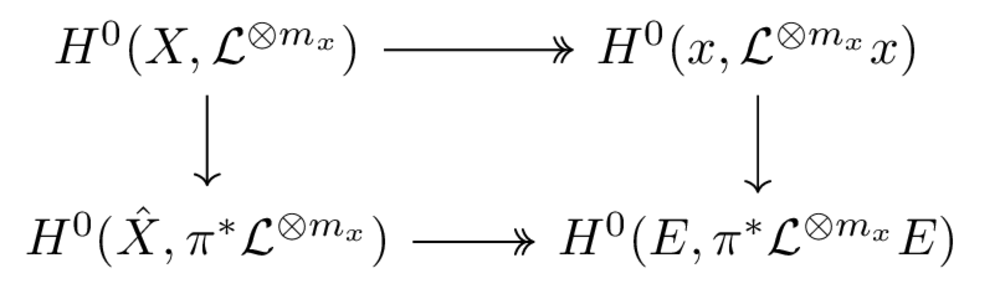
\includegraphics[width=0.50\textwidth]{../img/2017-12-10-kodaira-blowup.png}
\caption{Insert caption [fig:kodaira-blowup]}
\end{figure}

where the vertical arrows are isomorphic (easy to see, maybe the right one needs
Hartog). So one only needs to see that  \(H^0(\hat X,\pi^*\mathcal{L}^{\otimes m_x})
\twoheadrightarrow H^0(E,\restr{\pi^*\mathcal{L}^{\otimes m_x}}{E})\). Since \(E\) is
a divisor of \(\hat X\), one has
\$
0 \longrightarrow \mathcal{O}(E) \longrightarrow \mathcal{O}\(_{\hat\ \text{X}}\) \longrightarrow
\mathcal{O}\(_{\text{E}}\) \longrightarrow 0
\$
hence 
\[
0 \longrightarrow \mathcal{O}(E)\otimes\pi^* \mathcal{L}^{\otimes m_x} \longrightarrow \pi^* \mathcal{L}^{\otimes m_x} \longrightarrow
\restr{\pi^*\mathcal{L}^{\otimes m_x}}{E} \longrightarrow 0.
\]

It remains to prove that \(H^1(\hat X, \mathcal{O}(E)\otimes\pi^* \mathcal{L}^{\otimes
m_x})\), or by \ref{thm:Kodaira-vanishing}, that \(\mathcal{O}(E)\otimes\pi^*
\mathcal{L}^{\otimes m_x}\otimes K_{\hat X}^{-1} = \mathcal{O}(-nE)\otimes\pi^*
(\mathcal{L}^{\otimes m_x}\otimes K_X^{-1})\) is
positive, where we used the fact that \(K_{\hat X} = \pi^* K_X\otimes \mathcal{O}_{\hat
X}((n-1)E)\). 

Note that on \(\hat X \setminus E\), one can choose \(m_x\) large enough such that \(\mathcal{L}^{\otimes m_x}\otimes K_X^{-1}\times \mathcal{O}(-nE)\) is positive. It
remains to observe \(E\subset \hat X\) which is in fact \(\mathbb{CP}^{n-1}\). But \(\restr{\mathcal{O}(-E)}{E} \equiv \mathcal{O}(1)\) is positive, which concludes the proof.
\end{proof}


\section{An analytic proof by Donaldson}
\label{sec:org6ac4566}
Emacs 25.3.1 (Org mode 9.0.5)
\end{document}